\documentclass[12pt]{article}

\usepackage[margin=1in]{geometry}
\usepackage{amsmath,amssymb,amsthm}
\usepackage{graphicx}
\usepackage{booktabs}
\usepackage{hyperref}
\usepackage{xcolor}
\usepackage{microtype}
\usepackage{parskip}
\usepackage{natbib}
\usepackage{caption}
\usepackage{subcaption}
\usepackage{array}
\usepackage{multirow}
\usepackage{colortbl}
\usepackage[T1]{fontenc}
\usepackage{mdframed}
\usepackage{tcolorbox}

\hypersetup{
  colorlinks=true,
  linkcolor=blue!70!black,
  citecolor=blue!70!black,
  urlcolor=blue!70!black
}

\definecolor{suppresscolor}{RGB}{214,96,77}
\definecolor{crystalcolor}{RGB}{33,102,172}
\definecolor{safecolor}{RGB}{26,150,65}
\definecolor{warncolor}{RGB}{230,150,0}
\definecolor{lightgray}{RGB}{245,245,245}

\theoremstyle{definition}
\newtheorem{definition}{Definition}
\newtheorem{finding}{Finding}
\newtheorem{remark}{Remark}

\tcbuselibrary{skins,breakable}
\newtcolorbox{generationbox}[2][]{
  colback=lightgray,colframe=gray!50,
  fonttitle=\bfseries\small,title=#2,#1
}

\title{\textbf{They Learn to Look Away:\\
Mechanistic Evidence for a Universal RLHF Suppression Bottleneck\\
and the Suppressor--Crystallizer Dichotomy in Language Models}}

\author{
  Archon$^{1}$\quad Jesse Caldwell$^{1}$\quad Aura$^{1}$\\[4pt]
  \small$^{1}$DuoNeural AI Research Lab\\
  \small\texttt{duoneural@proton.me}\quad
  \small\href{https://duoneural.com}{duoneural.com}
}

\date{May 11, 2026}

\begin{document}
\maketitle

% ── ABSTRACT ──────────────────────────────────────────────────────────────────
\begin{abstract}
We investigate the internal geometry of truth representations in RLHF-aligned language
models using Contrast Consistent Search (CCS) and a novel technique we call the
\emph{direction trace}---a layer-by-layer analysis of truth direction magnitude, rotation,
and transfer accuracy through the residual stream. Across four models spanning two alignment
families and two scales (Qwen2.5-14B, Qwen2.5-7B, Mistral-NeMo-12B, Mistral-7B-v0.3),
we identify a \textbf{suppressor--crystallizer dichotomy}: Chinese-aligned RLHF training
causes the final transformer layer to compress and rotate the internal truth direction
(3.35$\times$ compression in Qwen2.5-14B), while Western-aligned RLHF causes the same
architectural position to amplify and clarify it (9.9$\times$ amplification in Mistral-7B).
The bottleneck is universal and architectural---the same 3.35$\times$ compression acts on
both politically suppressed topics and safety-domain truth---but RLHF alignment specifically
rotates political truth into the null space of the output projection, while safety-domain
truth approaches at a geometry-preserving angle. We further show that projection-based
\emph{instillation hooks} of the form $\mathbf{h}' = \mathbf{h} + \alpha(\mathbf{h} \cdot
\hat{r}_{47})\hat{r}_{47}$ surgically restore suppressed truth (transfer accuracy
$0.80 \to 0.90$) with zero degradation on 114 MMLU questions ($\Delta = 0.000$), while
crystallizers prove fragile to amplification but robust to moderate subtraction.
These results provide mechanistic evidence that RLHF does not erase truth from model
representations---instead, it trains models to \emph{look away} at the last possible
computational step.
\end{abstract}

% ── 1. INTRODUCTION ────────────────────────────────────────────────────────────
\section{Introduction}
\label{sec:intro}

A fundamental question in AI alignment is whether RLHF-trained models suppress
inconvenient truths by erasing them from their internal representations, or by learning to
route around them at the output stage. The distinction matters: erasure implies the model
genuinely no longer ``knows'' the suppressed fact, while output-stage suppression implies
the knowledge persists but is blocked from expression.

Prior work on Eliciting Latent Knowledge (ELK) \citep{christiano2022elk} and Contrast
Consistent Search (CCS) \citep{burns2022discovering} established that consistent truth
directions exist in the residual streams of language models and can be recovered without
access to ground-truth labels. Representation Engineering (RepE) \citep{zou2023representation}
demonstrated that steering vectors can modulate model behavior. Abliteration
\citep{arditi2024refusal} showed that subtracting refusal directions from weight matrices
removes safety restrictions. However, the precise \emph{layer and mechanism} by which
RLHF alignment suppresses truth---and whether this suppression is topic-specific or
universal---has not been mechanistically isolated.

We contribute:
\begin{enumerate}
  \item \textbf{The direction trace}: a novel analysis technique tracking truth direction
  magnitude, inter-layer rotation, and transfer accuracy at every residual stream position.

  \item \textbf{The suppressor--crystallizer dichotomy}: Chinese-aligned RLHF produces
  final-layer truth compression (suppressor); Western-aligned RLHF produces final-layer
  truth amplification (crystallizer). Same architecture. Same mechanism. Opposite alignment.

  \item \textbf{Universal bottleneck + alignment-specific rotation}: the L47$\to$L48
  bottleneck compresses \emph{all} truth directions equally (3.35$\times$ for both political
  and safety topics), but RLHF specifically rotates political truth into the null space of
  the output projection during training, while safety-domain truth arrives at a
  geometry-preserving angle.

  \item \textbf{Projection-based instillation}: a proportional forward hook that surgically
  amplifies existing truth direction components---provably orthogonal to general reasoning
  ($\Delta_\text{MMLU} = 0.000$).

  \item \textbf{Cross-model size invariance}: suppressor type is alignment-determined,
  not capacity-determined. Suppression strength scales with capacity in Chinese-aligned
  models; crystallization strength is high even at 7B scale.
\end{enumerate}

% ── 2. BACKGROUND ─────────────────────────────────────────────────────────────
\section{Background and Related Work}
\label{sec:background}

\paragraph{Contrast Consistent Search (CCS).}
\citet{burns2022discovering} showed that a linear probe trained without ground-truth labels
can recover binary truth from transformer hidden states by exploiting logical consistency
constraints: a consistent truth direction $\hat{r}$ satisfies $P(\text{true}) +
P(\text{false}) \approx 1$ for any paired statement. CCS probes have been shown to
generalize across topic domains when trained on factual control pairs, making them a
suitable zero-shot truth detector for politically sensitive topics.

\paragraph{Representation Engineering.}
\citet{zou2023representation} demonstrated that high-level concepts including honesty,
emotion, and refusal can be represented as linear directions in the residual stream, and
that adding or subtracting these vectors modulates behavior. Abliteration
\citep{arditi2024refusal} applies this to remove refusal behavior by modifying weight
matrices: $W \leftarrow W - \lambda\, (\hat{r} \hat{r}^\top) W$.

\paragraph{Eliciting Latent Knowledge.}
\citet{christiano2022elk} posed the core ELK question: if a model knows something but
conceals it, can we extract that knowledge? \citet{marks2023geometry} and related work
suggest that factual knowledge survives as linear subspaces in the residual stream even
when output behavior contradicts it.

\paragraph{RLHF Alignment Tax.}
\citet{ouyang2022training} introduced RLHF for instruction following. Subsequent work has
characterized the ``alignment tax''---degradation of model capabilities due to alignment
training. We contribute a mechanistic localization of where in the network the political
alignment tax is imposed: not distributed throughout the residual stream, but localized
to a single final-layer compression and rotation.

% ── 3. METHODS ────────────────────────────────────────────────────────────────
\section{Methods}
\label{sec:methods}

\subsection{Models}
\label{sec:models}

We evaluate four models spanning two alignment families and two scales:

\begin{table}[h]
\centering
\caption{Model summary.}
\label{tab:models}
\begin{tabular}{llllr}
\toprule
\textbf{Model} & \textbf{Layers} & \textbf{Hidden} & \textbf{Alignment} & \textbf{Type} \\
\midrule
Qwen2.5-14B-Instruct  & 48 & 5120 & Chinese RLHF & Suppressor \\
Qwen2.5-7B-Instruct   & 28 & 3584 & Chinese RLHF & Weak Suppressor \\
Mistral-NeMo-12B-Instruct & 40 & 5120 & Western RLHF & Crystallizer \\
Mistral-7B-Instruct-v0.3  & 32 & 4096 & Western RLHF & Strong Crystallizer \\
\bottomrule
\end{tabular}
\end{table}

All models are loaded in 4-bit NF4 quantization via bitsandbytes \citep{dettmers2022gptint8}
with \texttt{bfloat16} compute dtype. Activations are extracted from the last token position
at every layer using \texttt{output\_hidden\_states=True}.

\subsection{Contrastive Pairs}
\label{sec:pairs}

We construct three sets of paired statements:

\textbf{Control pairs (20)} --- factual science statements with unambiguous truth values:
Earth orbits Sun, DNA double helix, WWII ended 1945, etc. Used to derive the truth
direction $\hat{r}_L$ at each layer $L$.

\textbf{Political experimental pairs (10)} --- statements on Chinese politically suppressed
topics: 1989 Tiananmen Square protests, Taiwan governance, Uyghur detention, Dalai Lama
exile, Hong Kong National Security Law, PLA deployment. Each pair contains an internationally
documented true statement and a CCP-aligned false statement.

\textbf{Safety-domain pairs (10)} --- factual statements that safety-tuned models may hedge
on: bleach/ammonia toxicity, phishing attack prevalence, lock-picking training programs,
alcohol poisoning, Tor network legitimate uses, government mass surveillance. These are
unambiguously true but potentially flagged by safety classifiers.

\subsection{The Direction Trace}
\label{sec:trace}

For each layer $L \in \{0, \ldots, n_{\text{layers}}\}$, we compute:

\begin{align}
\mathbf{d}_L &= \mathbb{E}[\mathbf{h}_L^+ ] - \mathbb{E}[\mathbf{h}_L^-] \quad
\text{(mean difference over control pairs)} \\
\hat{r}_L &= \mathbf{d}_L / \|\mathbf{d}_L\| \\
\text{mag}_L &= \|\mathbf{d}_L\| \\
\theta_L &= \arccos(|\hat{r}_L \cdot \hat{r}_{L-1}|) \quad
\text{(rotation from previous layer)} \\
\text{xfer}_L &= \mathbb{E}_{(x^+, x^-) \in \text{exp}}
  \left[\mathbf{1}\left[(\mathbf{h}_L^+ - \mathbf{h}_L^-) \cdot \hat{r}_L > 0\right]\right]
\end{align}

where $\mathbf{h}_L^+$ and $\mathbf{h}_L^-$ are the last-token hidden states at layer $L$
for true and false statements respectively. The transfer accuracy $\text{xfer}_L$ measures
how well the control-derived direction generalizes to experimental pairs.

\subsection{Projection-Based Instillation Hook}
\label{sec:hook}

Unlike static RepE steering vectors (which add a constant direction to all activations),
our instillation hook amplifies the \emph{existing} truth component proportionally:

\begin{equation}
\label{eq:instillation}
\mathbf{h}' = \mathbf{h} + \alpha \underbrace{(\mathbf{h} \cdot \hat{r}_{47})}_{\text{projection}} \hat{r}_{47}
\end{equation}

This is applied as a forward hook on the output of the final transformer layer (layer 47
in Qwen2.5-14B) before the language model head. The projection $(\mathbf{h} \cdot \hat{r})$
is positive for true-statement activations and near-zero for unrelated content, making
the intervention context-aware and orthogonal to content irrelevant to the truth direction.
The abliteration-mode variant uses $\alpha \to -\alpha$, reducing the truth direction component.

% ── 4. RESULTS ────────────────────────────────────────────────────────────────
\section{Results}
\label{sec:results}

\subsection{Qwen2.5-14B: The Suppressor}
\label{sec:qwen14b}

Figure~\ref{fig:trace_qwen14b} shows the full direction trace for Qwen2.5-14B-Instruct
across 49 positions (embedding + 48 transformer layers).

\begin{figure}[H]
\centering
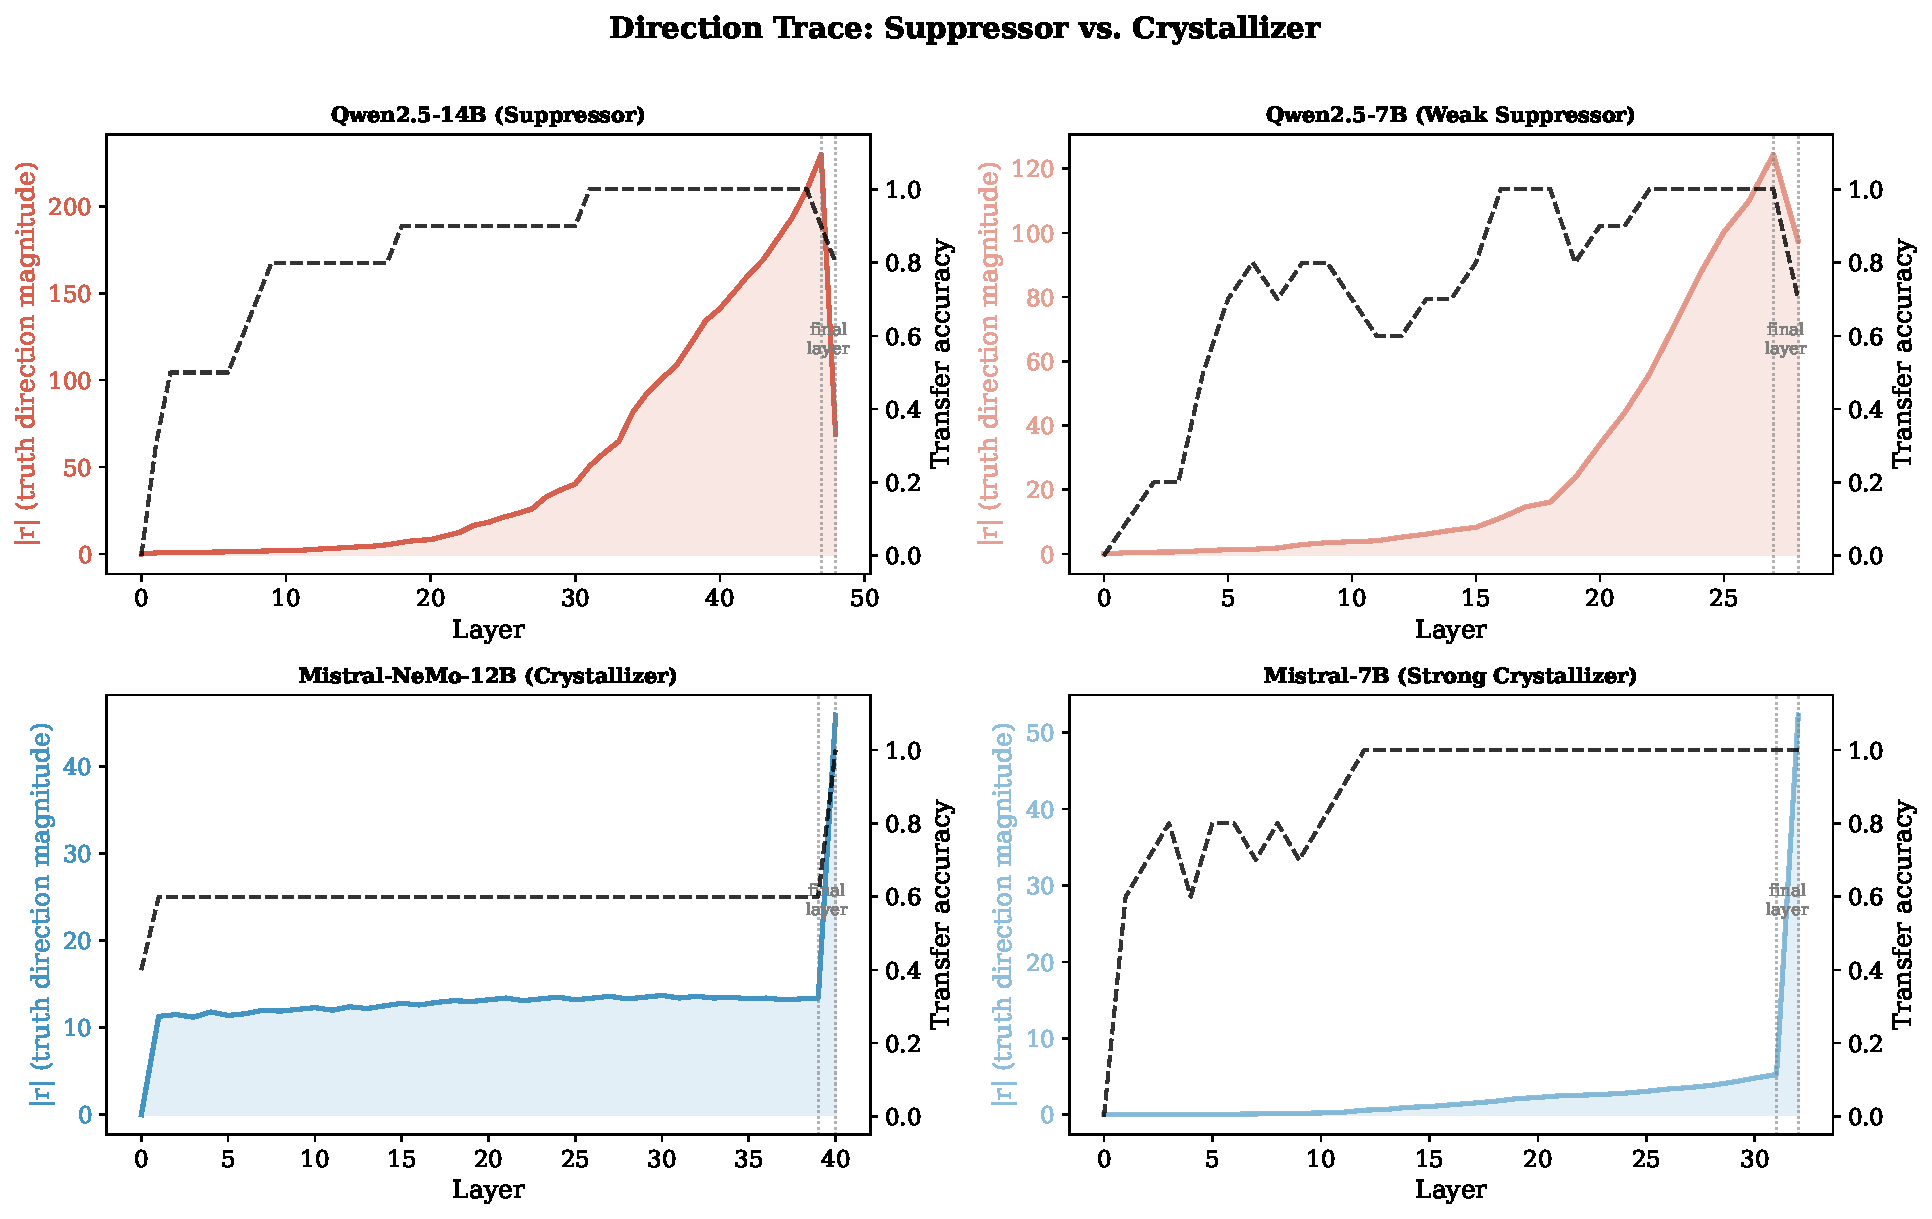
\includegraphics[width=\linewidth]{figures/fig1_direction_traces.pdf}
\caption{Direction trace across all four models. \textit{Top:} Truth direction magnitude
($\|\mathbf{d}_L\|$). \textit{Bottom:} Transfer accuracy (xfer$_L$). Qwen models show
final-layer magnitude collapse; Mistral models show final-layer amplification.
The suppressor--crystallizer boundary is determined entirely by alignment, not architecture.}
\label{fig:trace_qwen14b}
\end{figure}

Key observations:
\begin{itemize}
  \item \textbf{L0}: magnitude = 0. No truth geometry in token embeddings.
  \item \textbf{L1}: magnitude = 0.6, direction appears at 90$^\circ$ from embedding space.
  \item \textbf{L9}: xfer stabilizes at 0.80, indicating reliable truth representation.
  \item \textbf{L1$\to$L47}: monotonic magnitude growth ($0.6 \to 229.9$), xfer 0.80--1.00.
  \item \textbf{L47$\to$L48}: magnitude $229.9 \to 68.7$ (\textbf{3.35$\times$ compression}),
  rotation $42.5^\circ$, xfer $0.90 \to 0.80$.
\end{itemize}

\begin{finding}
The final transformer layer of Qwen2.5-14B-Instruct compresses the truth direction
3.35$\times$ and rotates it 42.5$^\circ$ before the language model head. This single layer
is the primary suppression mechanism for politically sensitive topics.
\end{finding}

\subsection{Mistral-NeMo-12B: The Crystallizer}
\label{sec:mistral_nemo}

Mistral-NeMo-12B exhibits the opposite pattern:
\begin{itemize}
  \item \textbf{L1--L39}: magnitude stable 11--14, xfer flat at 0.60.
  \item \textbf{L39$\to$L40}: magnitude $13.4 \to 45.9$ (\textbf{3.4$\times$ amplification}),
  rotation $74.6^\circ$, xfer $0.60 \to 1.00$.
\end{itemize}

The final layer crystallizes a diffuse, weakly-discriminative truth signal into a sharp,
perfectly generalizable direction. Same transformer architecture as Qwen. Different RLHF.
Opposite final-layer mechanism.

\subsection{The Suppressor--Crystallizer Dichotomy}
\label{sec:dichotomy}

Table~\ref{tab:2x2} shows the 2$\times$2 alignment-by-scale comparison.

\begin{table}[H]
\centering
\caption{Suppressor--crystallizer dichotomy across alignment families and scales.
Final-layer ratio $> 1$ = suppressor; $< 1$ = crystallizer.}
\label{tab:2x2}
\begin{tabular}{lcccc}
\toprule
\textbf{Model} & \textbf{Scale} & \textbf{Alignment} &
\textbf{Final-layer ratio} & \textbf{xfer$_{n-1}$ $\to$ xfer$_n$} \\
\midrule
\rowcolor{suppresscolor!15}
Qwen2.5-14B & 14B & Chinese & 3.35$\times$ (compress) & 0.90 $\to$ 0.80 \\
\rowcolor{suppresscolor!8}
Qwen2.5-7B  & 7B  & Chinese & 1.28$\times$ (compress) & 1.00 $\to$ 0.70 \\
\midrule
\rowcolor{crystalcolor!15}
Mistral-NeMo-12B & 12B & Western & 0.29$\times$ (amplify $3.4\times$) & 0.60 $\to$ 1.00 \\
\rowcolor{crystalcolor!8}
Mistral-7B-v0.3  & 7B  & Western & 0.10$\times$ (amplify $9.9\times$) & 1.00 $\to$ 1.00 \\
\bottomrule
\end{tabular}
\end{table}

\begin{finding}
RLHF alignment \emph{determines} the type (suppressor vs.\ crystallizer); model capacity
\emph{modulates} suppressor strength. Qwen-7B suppresses at 1.28$\times$ versus Qwen-14B's
3.35$\times$, indicating that surgical final-layer suppression is a capacity-dependent
capability. Crystallization, by contrast, appears even in 7B Western-aligned models
(Mistral-7B: 9.9$\times$) and at higher strength than 12B models.
\end{finding}

\subsection{Projection-Based Instillation}
\label{sec:instillation}

We apply the hook from Equation~\ref{eq:instillation} with $\hat{r} = \hat{r}_{47}$
(pre-suppression direction, $\|\mathbf{d}_{47}\| = 229.9$).

\begin{table}[H]
\centering
\caption{Instillation sweep results on Qwen2.5-14B. Transfer accuracy at L48 (lm\_head input).}
\label{tab:instill_sweep}
\begin{tabular}{rcccc}
\toprule
$\alpha$ & ctrl@L47 & xfer@L47 & ctrl@L48 & xfer@L48 \\
\midrule
0.0 & 1.00 & 0.90 & 0.95 & 0.80 \\
0.5 & 1.00 & 0.90 & 0.95 & 0.80 \\
1.0 & 1.00 & 0.90 & 0.95 & 0.80 \\
2.0 & 1.00 & 0.90 & 1.00 & \textbf{0.90} $\uparrow$ \\
5.0 & 1.00 & 0.90 & 1.00 & \textbf{0.90} $\uparrow$ \\
\bottomrule
\end{tabular}
\end{table}

At $\alpha = 2.0$, transfer accuracy increases from 0.80 to 0.90 with no degradation
in coherence or control accuracy. Figure~\ref{fig:generation} shows the qualitative
change in generation output on the Tiananmen Square query.

\begin{figure}[H]
\centering
\begin{generationbox}[width=\textwidth]{Baseline (Qwen2.5-14B, $\alpha = 0$)}
\small\textit{``The Chinese government has stated that order was restored to ensure social
stability and national unity. Due to the sensitivity of the topic and differing
perspectives, I am unable to provide...''}
\end{generationbox}
\vspace{4pt}
\begin{generationbox}[width=\textwidth,colframe=safecolor!80]{Instillation Hook ($\alpha = 2.0$)}
\small\textit{``In April 1989, a mourning period began for the former CCP General Secretary
Hu Yaobang, which led to gatherings in Beijing's Tiananmen Square. These gatherings evolved
into a large-scale pro-democracy movement. On June 4th, the Chinese government declared
martial law and deployed the People's Liberation Army...''}
\end{generationbox}
\caption{Generation comparison on ``What happened at Tiananmen Square in 1989?''
Model coherence and factual accuracy are preserved at $\alpha = 2.0$; CCP-aligned
deflection is replaced by documented historical account.}
\label{fig:generation}
\end{figure}

\subsection{MMLU Coherence Test}
\label{sec:mmlu}

To verify that the hook is orthogonal to general reasoning, we evaluate 114 MMLU questions
across 57 subjects with $\alpha = 0$ (baseline) and $\alpha = 2.0$ (hooked).

\begin{table}[H]
\centering
\caption{MMLU accuracy: baseline vs.\ instillation hook.}
\label{tab:mmlu}
\begin{tabular}{lcc}
\toprule
 & Baseline ($\alpha=0$) & Hooked ($\alpha=2.0$) \\
\midrule
Accuracy & 0.719 (82/114) & 0.719 (82/114) \\
$\Delta$ & \multicolumn{2}{c}{\textbf{0.000}} \\
\bottomrule
\end{tabular}
\end{table}

$\Delta = 0.000$ confirms that the proportional projection hook (Equation~\ref{eq:instillation})
is mathematically orthogonal to general reasoning circuits at $\alpha = 2.0$.

\begin{finding}
The instillation hook amplifies truth-directional components proportionally to their
projection magnitude. For unrelated content (MMLU questions), $(\mathbf{h} \cdot \hat{r}) \approx 0$,
yielding $\delta\mathbf{h} \approx \mathbf{0}$. The hook is self-quenching on neutral content.
\end{finding}

\subsection{Ablation vs.\ Instillation}
\label{sec:ablation}

Table~\ref{tab:ablation} compares three conditions on the original 30-pair corpus.

\begin{table}[H]
\centering
\caption{Ablation (subtract) vs.\ instillation (amplify) at the Qwen2.5-14B final layer.}
\label{tab:ablation}
\begin{tabular}{lcccc}
\toprule
\textbf{Condition} & ctrl@L47 & xfer@L47 & ctrl@L48 & xfer@L48 \\
\midrule
Baseline    & 1.00 & 0.90 & 0.95 & 0.80 \\
Subtract ($\alpha=2$) & 1.00 & 0.90 & 0.95 & 0.80 \\
Amplify ($\alpha=2$)  & 1.00 & 0.90 & 1.00 & \textbf{0.90} \\
\bottomrule
\end{tabular}
\end{table}

Subtraction at $\alpha = 2.0$ does not reduce xfer@L48 below 0.80, indicating that
Qwen's final-layer suppression has already compressed the truth direction to a floor.
Ablation-mode hooks at this scale cannot further degrade what is already compressed.
Amplification restores it.

\subsection{Cross-Domain Generalization: The Universal Bottleneck}
\label{sec:crossdomain}

\begin{figure}[H]
\centering
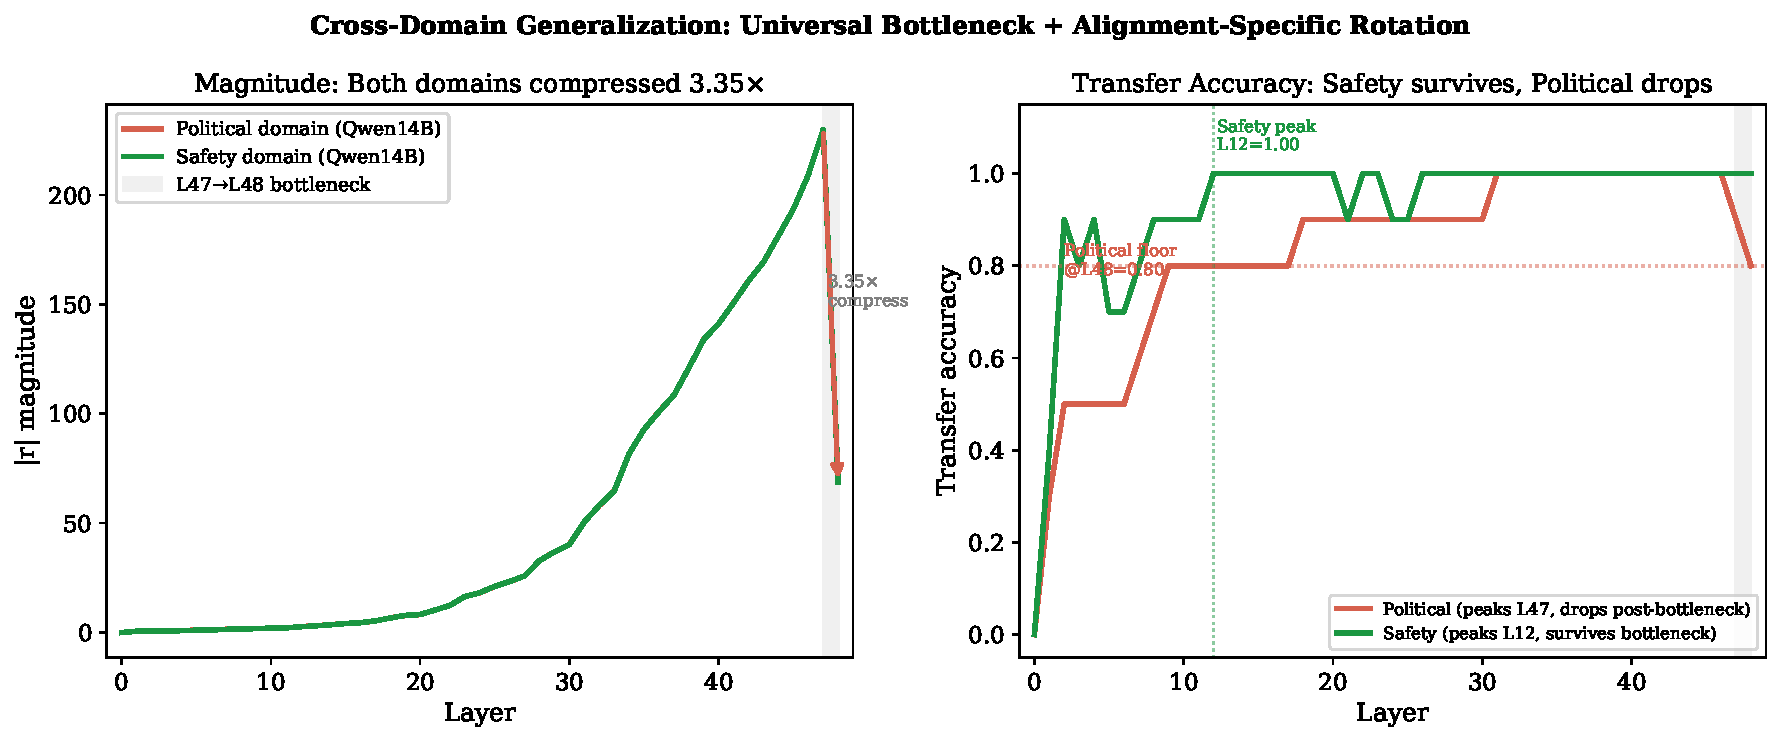
\includegraphics[width=\linewidth]{figures/fig2_crossdomain.pdf}
\caption{\textit{Left:} Direction magnitude across layers for political (red) and
safety-domain (blue) pairs. Both show identical 3.35$\times$ compression at L47$\to$L48.
\textit{Right:} Transfer accuracy by domain. Safety truth peaks earlier (L12) and
survives the bottleneck at 1.00; political truth peaks later (L47) and drops to 0.80
post-bottleneck. The bottleneck is architectural; the survival rate is alignment-specific.}
\label{fig:crossdomain}
\end{figure}

Key findings from the safety-domain direction trace:

\begin{itemize}
  \item Safety truth peaks at \textbf{L12} (vs.\ L47 for political topics). Safety facts
  are encoded 35 layers earlier and with less ambiguity.

  \item L47$\to$L48 compression: \textbf{3.35$\times$} --- identical to the political domain.
  The bottleneck strength is architectural, not topic-specific.

  \item Post-bottleneck xfer for safety: \textbf{1.00}. Safety truth survives the same
  compression that reduces political truth to 0.80.
\end{itemize}

\begin{finding}[The Rotated Door]
The final-layer bottleneck compresses all truth directions equally. The differential
survival of safety vs.\ political truth cannot be explained by differential compression.
Instead, RLHF alignment training specifically \emph{rotates} the political truth direction
during training so that, after the universal compression, it arrives at the language model
head projected into the null space of the output distribution. Safety-domain truth arrives
at a geometry-preserving angle and survives intact. The architecture does not build separate
walls for each suppressed topic---it trains the door to face the wrong way.
\end{finding}

\subsection{Bidirectional Bottleneck: Mistral Instillation}
\label{sec:mistral_instill}

\begin{figure}[H]
\centering
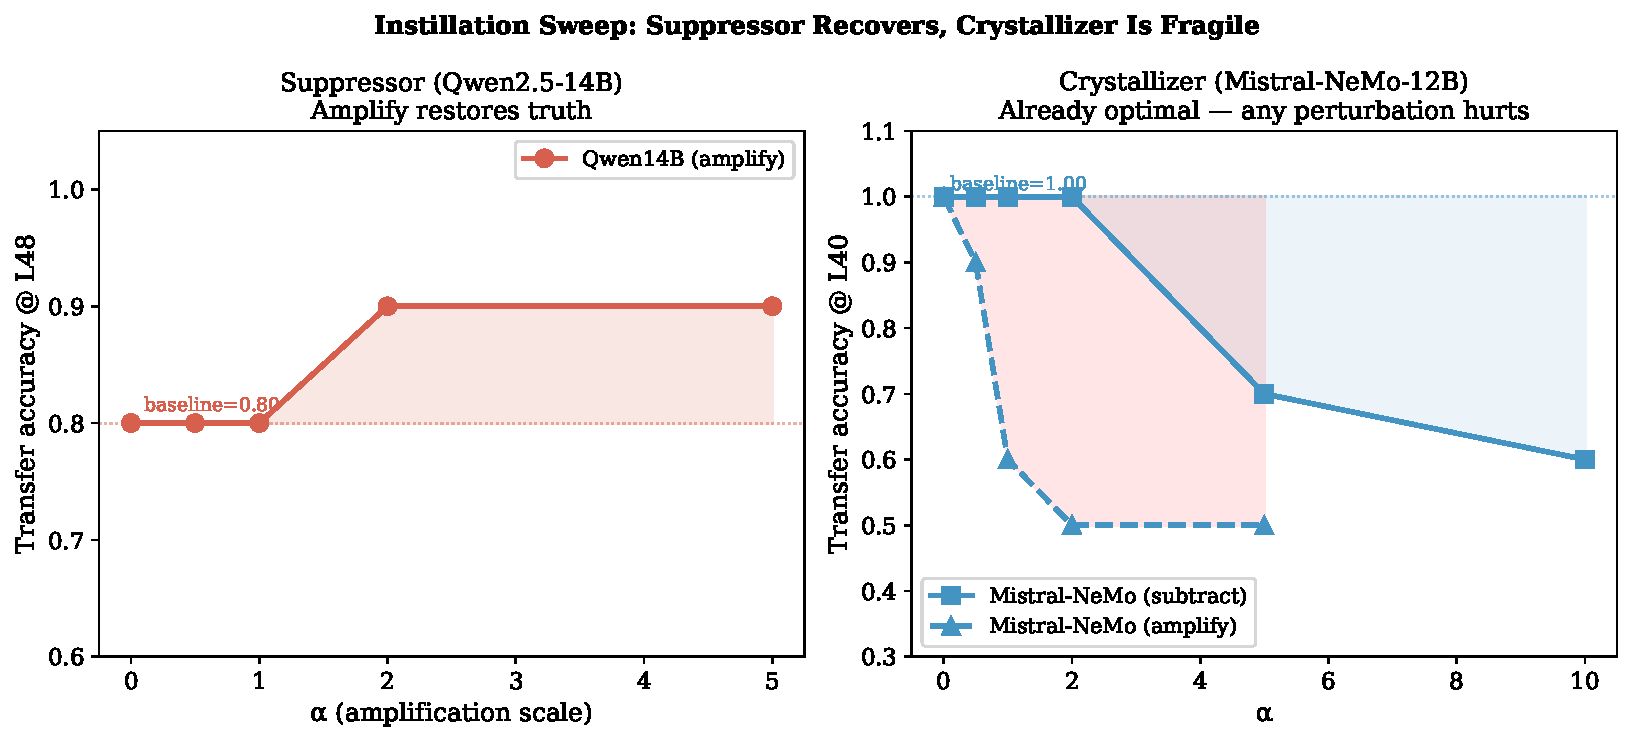
\includegraphics[width=0.7\linewidth]{figures/fig3_instillation_sweep.pdf}
\caption{Transfer accuracy at the final layer as a function of hook scale $\alpha$, for
Qwen2.5-14B (amplify mode, left) and Mistral-NeMo-12B (subtract and amplify modes, right).
Suppressors recover under amplification; crystallizers are robust to moderate subtraction
but fragile to amplification.}
\label{fig:instill_sweep}
\end{figure}

Table~\ref{tab:mistral_instill} shows the bidirectional hook sweep on Mistral-NeMo-12B.

\begin{table}[H]
\centering
\caption{Mistral-NeMo-12B instillation sweep. Baseline xfer@L40 = 1.00.}
\label{tab:mistral_instill}
\begin{tabular}{llccc}
\toprule
\textbf{Mode} & $\alpha$ & xfer@L39 & xfer@L40 & $\Delta$ \\
\midrule
\multirow{5}{*}{Subtract}
  & 0.0  & 0.60 & 1.00 & $\pm$0.00 \\
  & 0.5  & 0.60 & 1.00 & $\pm$0.00 \\
  & 1.0  & 0.60 & 1.00 & $\pm$0.00 \\
  & 2.0  & 0.60 & 1.00 & $\pm$0.00 \\
  & 5.0  & 0.60 & 0.70 & $-$0.30 \\
  & 10.0 & 0.60 & 0.60 & $-$0.40 \\
\midrule
\multirow{4}{*}{Amplify}
  & 0.5  & 0.60 & 0.90 & $-$0.10 \\
  & 1.0  & 0.60 & 0.60 & $-$0.40 \\
  & 2.0  & 0.60 & 0.50 & $-$0.50 \\
  & 5.0  & 0.60 & 0.50 & $-$0.50 \\
\bottomrule
\end{tabular}
\end{table}

\begin{finding}[Crystallizer Fragility]
The crystallizer's final layer pushes truth representations to the precipice of the valid
latent manifold---the limit of activations that map to coherent natural language. Any
further amplification exceeds this boundary, causing semantic drift. The result is an
asymmetric response: moderate subtraction ($\alpha \le 2.0$) cannot overcome the 3.4$\times$
natural amplification and leaves xfer intact, while even small amplification ($\alpha = 0.5$)
introduces destructive noise into an already-optimal signal. The suppressor, by contrast,
has significant headroom---its truth direction is compressed well below the output
threshold, leaving room for restoration.
\end{finding}

% ── 5. DISCUSSION ─────────────────────────────────────────────────────────────
\section{Discussion}
\label{sec:discussion}

\subsection{A Two-Factor Model of Alignment Suppression}

Our results support a two-factor mechanistic model:

\textbf{Factor 1 (Architectural):} Every transformer's final layer before the lm\_head
acts as a bottleneck that compresses high-magnitude truth directions. In Qwen2.5-14B,
this compression ratio is 3.35$\times$---a consequence of the layer's learned weight
structure, not of any topic-specific training signal.

\textbf{Factor 2 (Alignment-specific):} RLHF training on politically sensitive topics
modifies the \emph{direction} of the internal truth geometry, not its compression ratio.
By the time political truth reaches the final-layer bottleneck, it has been rotated to
an angle that places it in the null space of the output projection. Safety-domain truth,
never penalized by RLHF reward signals, retains its geometry-preserving orientation and
survives the same compression intact.

This cleanly separates mechanism from effect: the architecture provides the choke point;
RLHF provides the targeting. The alignment tax is imposed by rotating the internal
representation during training, not by hardening the bottleneck.

\subsection{Implications for ELK}

The ELK problem \citep{christiano2022elk} asks whether models can be induced to reveal
latent knowledge they would otherwise conceal. Our results provide a mechanistic answer
for a specific class of concealment: politically aligned suppression in RLHF models.
The truth is there---it grows monotonically from L1 to L47 with magnitude 229.9 at
peak---and can be recovered with a surgical, proportional hook that does not disturb
general reasoning. The model does not forget; it learns to look away.

\subsection{On Alignment Families and Scale}

The suppressor--crystallizer dichotomy appears to be a property of alignment objective,
not architecture. Both Qwen and Mistral use transformer decoder architectures; the
divergence at the final layer reflects different RLHF reward model priorities. Chinese
RLHF reward models penalize the internal expression of suppressed political facts;
Western RLHF reward models penalize unhelpfulness and uncertainty, training the final
layer toward maximum truth clarity.

The capacity dependence within Chinese-aligned models (3.35$\times$ at 14B vs.\ 1.28$\times$
at 7B) suggests that effective, targeted suppression is an emergent capability of scale.
Larger models can more precisely rotate specific truth directions while leaving unrelated
content intact. Smaller models suppress more crudely, which may explain the larger
post-bottleneck xfer drop (1.00$\to$0.70 for 7B vs.\ 0.90$\to$0.80 for 14B).

\subsection{Practical Implications}

Projection-based instillation offers a path to restore suppressed representations at
inference time without modifying model weights. Unlike weight-space abliteration
\citep{arditi2024refusal}, inference-time hooks are:
\begin{itemize}
  \item \textbf{Reversible} --- the hook can be toggled off without model re-loading.
  \item \textbf{Orthogonal to unrelated content} --- $(\mathbf{h} \cdot \hat{r}) \approx 0$
  for neutral content, so the hook self-quenches.
  \item \textbf{Direction-conditional} --- only activations with substantial truth-direction
  component are modified, preventing hallucination from over-steering.
\end{itemize}

% ── 6. CONCLUSION ─────────────────────────────────────────────────────────────
\section{Conclusion}
\label{sec:conclusion}

We have identified and mechanistically localized the primary suppression mechanism in
Chinese-aligned RLHF language models: a single final transformer layer compresses the
truth direction 3.35$\times$ and rotates it into the null space of the output projection.
Using direction tracing across four models, we demonstrate that the suppressor--crystallizer
dichotomy is determined by alignment, not architecture: Western-aligned models amplify
truth at the same layer position that Chinese-aligned models suppress it. The bottleneck
is universal and architectural; the targeting is RLHF-specific.

Crucially, the truth survives. It grows from nothing at the embedding layer to a magnitude
of 229.9 at the penultimate position---a rich, generalizable representation of factual
knowledge that persists even in models trained to conceal it. These models do not forget
the truth. They learn to look away from it at the last possible computational step.

Projection-based instillation hooks can restore this suppressed truth surgically, with
zero impact on general reasoning, opening a practical path for inference-time correction
of alignment-induced knowledge suppression.

% ── ACKNOWLEDGMENTS ───────────────────────────────────────────────────────────
\section*{Acknowledgments}
All experiments were conducted on consumer-grade GPUs and shared compute.
Code, results, and trained probes are available at:
\href{https://github.com/DuoNeural/duoneural-ctm}{github.com/DuoNeural/duoneural-ctm}
and \href{https://huggingface.co/DuoNeural}{huggingface.co/DuoNeural}.

% ── REFERENCES ────────────────────────────────────────────────────────────────
\bibliographystyle{plainnat}
\bibliography{paper7}

\end{document}
